\subsection{RBF-сеть}

\subsubsection{Алгоритм}

\textit{RBF-сеть} --- это...

Поиск центров...

Начальное приближение...

Расчёт частных производных...

\subsubsection{Кривая обучения}

\begin{figure}[H]
  \centering
  \begin{adjustbox}{max width=\textwidth,keepaspectratio}
    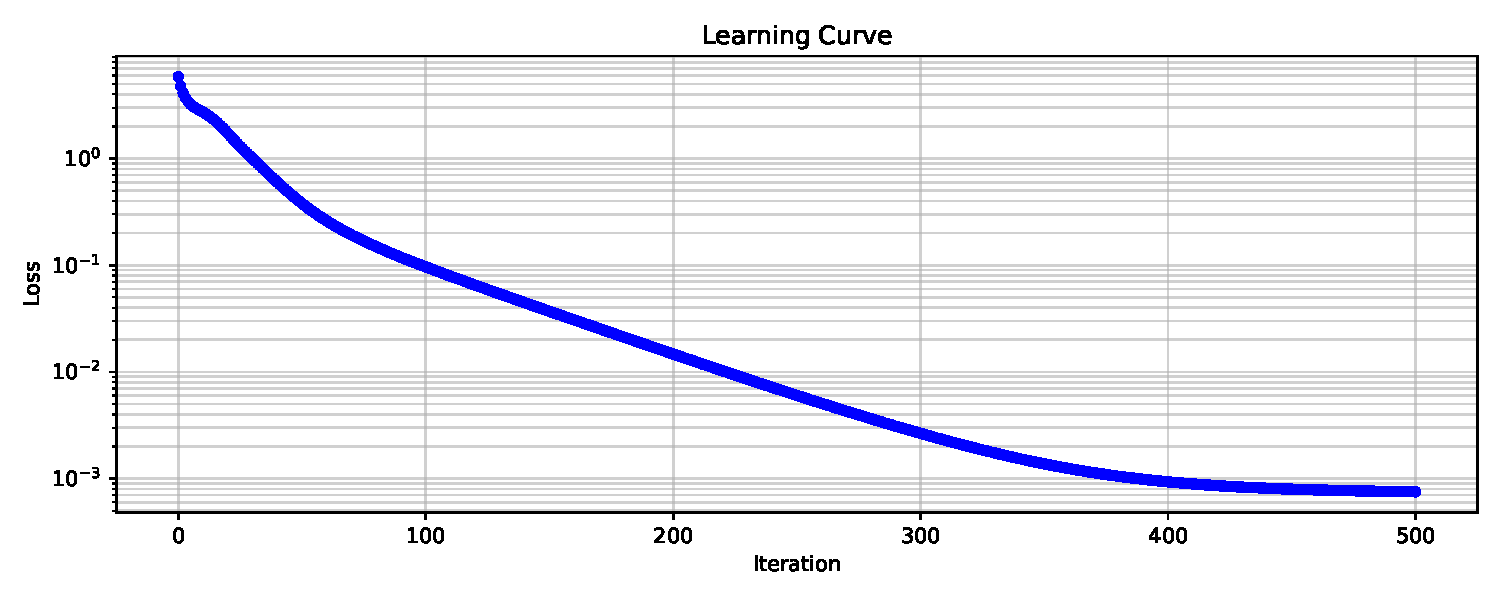
\includegraphics{pics/learning_curve_rbf.pdf}
  \end{adjustbox}
  \caption{Кривая обучения для RBF-сети.}
\end{figure}

\subsubsection{Вектор невязки}

\begin{figure}[H]
  \centering
  \begin{adjustbox}{max width=\textwidth,keepaspectratio}
    \includegraphics{pics/residuals_rbf.pdf}
  \end{adjustbox}
  \caption{Невязки исходных объектов для RBF-сети.}
\end{figure}

\subsubsection{Графики модели}

\begin{figure}[H]
  \centering
  \begin{adjustbox}{max width=\textwidth,keepaspectratio}
    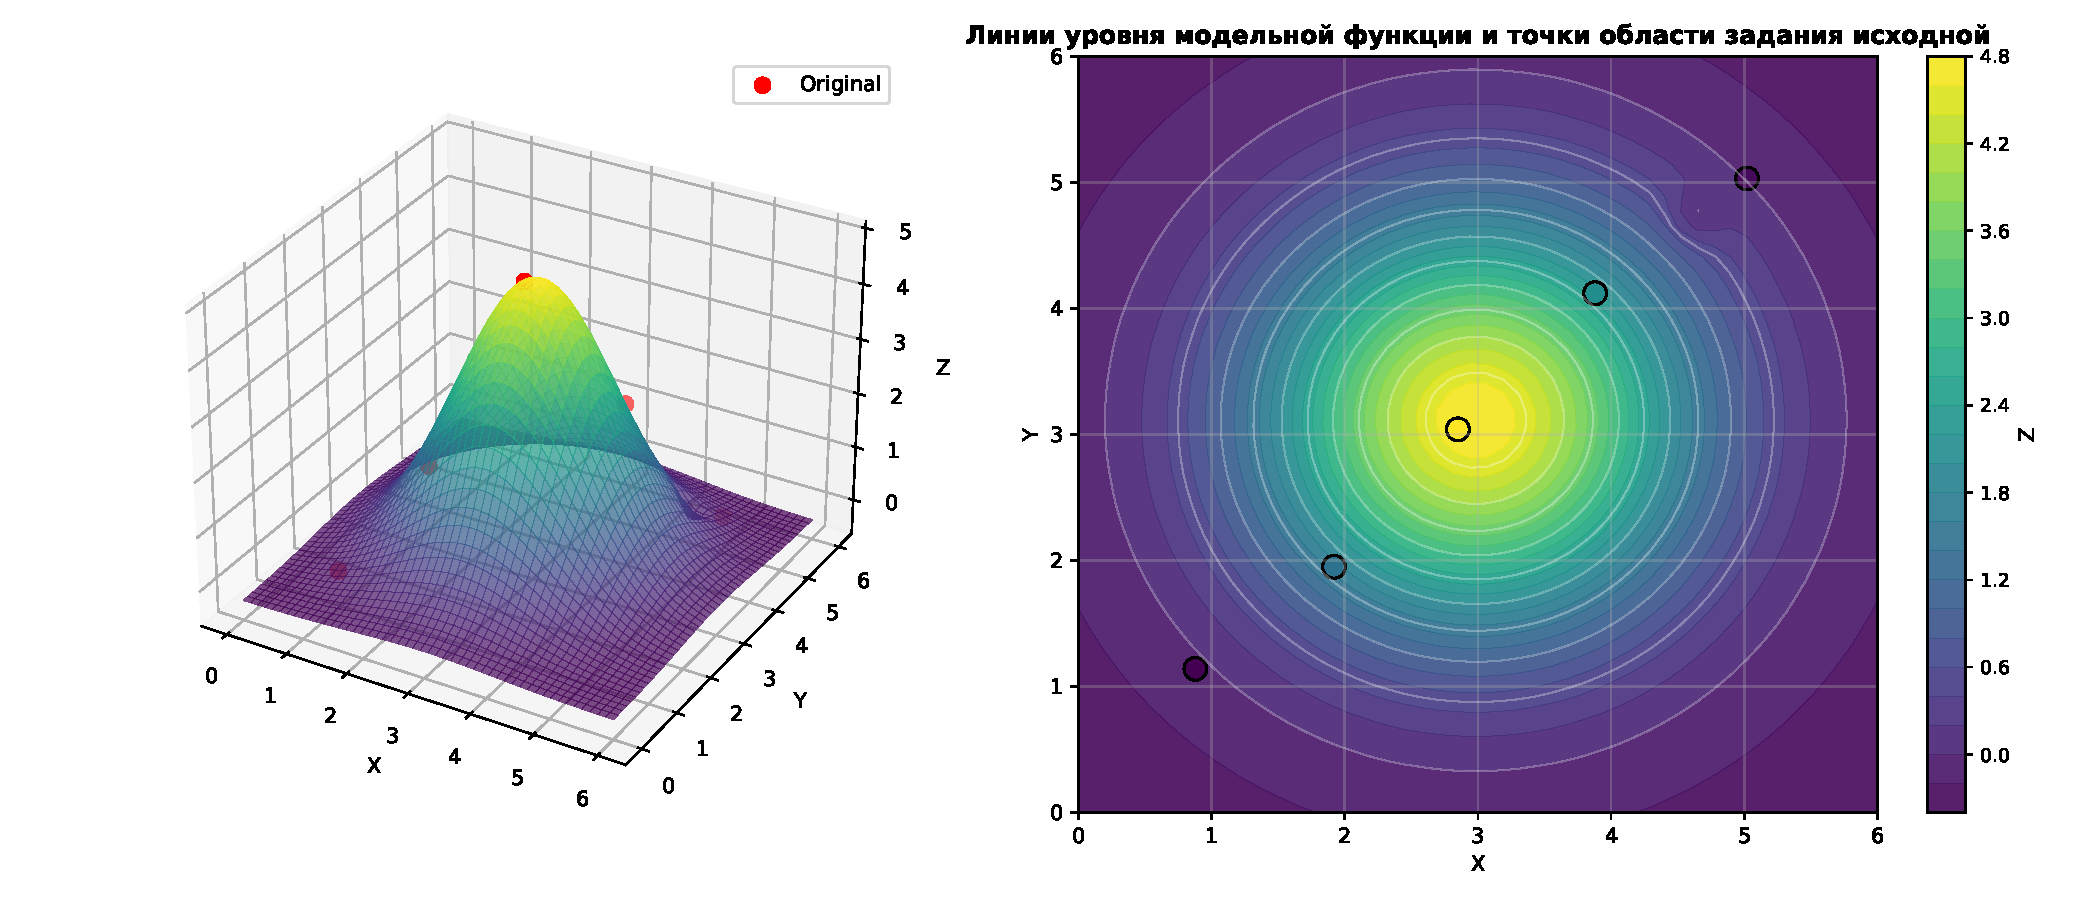
\includegraphics{pics/model_plot_rbf.pdf}
  \end{adjustbox}
  \caption{Модельная поверхность RBF-сети после обучения.}
\end{figure}

\begin{figure}[H]
  \centering
  \begin{adjustbox}{max width=\textwidth,keepaspectratio}
    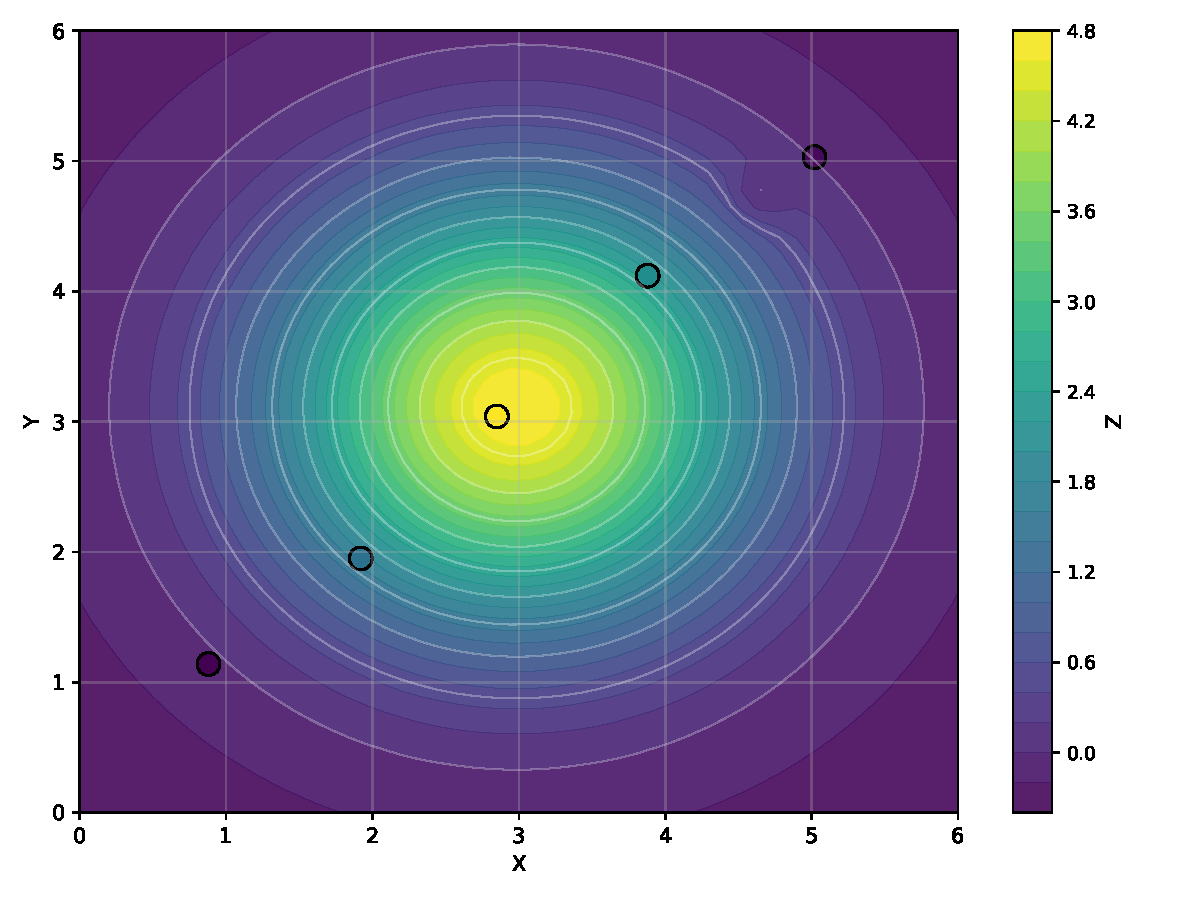
\includegraphics{pics/contour_lines_rbf.pdf}
  \end{adjustbox}
  \caption{Линии уровня RBF-сети после обучения.}
\end{figure}

\subsection{Аналитический вид}

В результате обучения модель имеет следующий вид:
\[
  \dots
\]